\documentclass{beamer}
%\documentclass[notes]{beamer}
%\documentclass[notes=only]{beamer}

\usepackage{tikz}
\usepackage{gitdags}
\usepackage{wrapfig}
\usepackage{xcolor}
\usepackage{xcolor-solarized}
\usepackage{soul}

\usetheme{Antibes}
\usecolortheme{dolphin}

\newcommand\gitcmd[1]{\texttt{git #1}}
\newcommand\gitsubcmd[1]{\texttt{#1}}
\newcommand\gflag[1]{\texttt{#1}}
\newcommand\grefspec[1]{\texttt{#1}}
\newcommand\gbranch[1]{\texttt{#1}}
\newcommand\gremotebranch[1]{\texttt{#1}}
\newcommand\gtag[1]{\texttt{#1}}
\newcommand\gHEAD{\texttt{HEAD}}
\newcommand\gremote[1]{\texttt{#1}}
\newcommand\goal[1]{\textbf{Goal:} #1}
\newcommand\defaultrepo{%
  \begin{figure}
    \centering
    \begin{tikzpicture}
      \gitDAG{
        A -- B -- {
          D,
          C -- E
        }
      };
      \gitbranch{master}
      {above=of D} {D}
      \gitbranch{topic}
      {above=of E} {E}
      \gitHEAD
      {above=of topic} {topic}
    \end{tikzpicture}
  \end{figure}
}

\title{Understanding Git}
\author{Johann Tutor}
\date{June 22, 2018}

\makeatletter
\hypersetup{
  pdftitle={\@title (\@date)},
  pdfauthor={\@author}
}
\makeatother

\begin{document}
\frame{\titlepage\begin{center}\includegraphics[height=\baselineskip]{cc-by-sa.eps}\end{center}}

%%%%%%%%%%%%%%%%%%%%%%%%%%%%%%%%%%%%%%%%%%%%%%%%%%%%%%%%%%%%%%%%%%%%%%
%%%%%%%%%%%%%%%%%%%%%%%%%%%%%%%%%%%%%%%%%%%%%%%%%%%%%%%%%%%%%%%%%%%%%%
\section{Introduction}

\begin{frame}
  \frametitle{Aims}
  By the end of this presentation, you should be able to:
  \begin{itemize}
    \item Read Git graphs.
    \item Visualize actions done on a Git repository.
    \item Understand what commits and branches are and how they interact.
  \end{itemize}
\end{frame}

\begin{frame}
  \frametitle{Assumptions}
  \begin{itemize}
    \item You are familiar enough with Git commands to use them.
    \item You understand the Git workflow (\gitsubcmd{add}, \gitsubcmd{commit}, \gitsubcmd{push}, etc.).
    \item You have a vague idea of what commits and branches are.
  \end{itemize}
\end{frame}

\begin{frame}
  \frametitle{What is Git?}
  \framesubtitle{``The stupid content tracker''}
  \begin{itemize}
    \item A distributed version control system (DVCS).
    \item Created in 2005 by Linus Torvalds to replace BitKeeper for Linux kernel development.
    \item Not GitHub.
  \end{itemize}
  \vfill
  \begin{block}{\texttt{man git}}
    ``Git is a fast, scalable, distributed revision control system with an
    unusually rich command set that provides both high-level operations and
    full access to internals.''
  \end{block}
\end{frame}

\begin{frame}
  \frametitle{Reading Git graphs}
  Git repositories are often represented using a directed acyclic graph (DAG).
  \begin{figure}
    \centering
    \begin{tikzpicture}
      \gitDAG{
        {Commit A} -- {Commit B} -- {
          D,
          C -- E
        } -- {Merge commit}
      };
      \gittag{tag}
      {above=of Commit B} {Commit B}
      \gitbranch{branch1}
      {above=of Merge commit} {Merge commit}
      \gitremotebranch{remote/branch1}
      {above=of D} {D}
      \gitbranch{branch2}
      {right=of E} {E}
      \gitHEAD
      {left=of branch1} {branch1}
    \end{tikzpicture}
  \end{figure}
  \vfill
  \begin{block}{Arrows}
    The arrows point to the commit's parent(s), not the flow of time.
  \end{block}
\end{frame}

\begin{frame}
  \frametitle{Our reference repository}
  \defaultrepo
\end{frame}

%%%%%%%%%%%%%%%%%%%%%%%%%%%%%%%%%%%%%%%%%%%%%%%%%%%%%%%%%%%%%%%%%%%%%%
%%%%%%%%%%%%%%%%%%%%%%%%%%%%%%%%%%%%%%%%%%%%%%%%%%%%%%%%%%%%%%%%%%%%%%
\section{Commits}

\begin{frame}
  \frametitle{What is a commit?}
  \begin{itemize}
    \item Commits record the changes of a repository.
    \item Commits also include a message, a timestamp (usually of creation), and an author.
    \item Except for the first commit, commits reference one or more parent commits.
    \item Commits are identified by a SHA-1 hash. This hash can be abbreviated to its unique prefix (usually 7).
    \item The bulk of the Git model is the DAG of commits.
  \end{itemize}
\end{frame}

\begin{frame}
  \frametitle{What is a commit?}
  In our reference repository, objects \grefspec{A} through \grefspec{E} are all commits.
  \defaultrepo
\end{frame}

\begin{frame}
  \frametitle{Committing}
  Committing occurs in two steps:
  \begin{enumerate}
    \item Staging: moving changes from the working tree into the staging area.
    \item Committing: recording changes from the staging area into a commit.
  \end{enumerate}
  \begin{figure}
    \centering
    \begin{tikzpicture}
      \SAandWT
    \end{tikzpicture}
  \end{figure}
  \vfill
  \begin{block}{Working tree}
    The tree of actual checked-out files.
  \end{block}
\end{frame}

%%%%%%%%%%%%%%%%%%%%%%%%%%%%%%%%%%%%%%%%%%%%%%%%%%%%%%%%%%%%%%%%%%%%%%
\subsection{\gitcmd{add}}

\begin{frame}
  \frametitle{\gitcmd{add}}
  \framesubtitle{``Add file contents to the index''}
  \begin{itemize}
    \item Stages changes to commit.
    \item Files can be selectively staged by specifying them as arguments.
    \item Hunks can be selectively staged by specifying the \gflag{-p} flag.
  \end{itemize}
  \vfill
  \begin{block}{Changes after staging}
    If changes are made to a file after the file has been staged, the new changes are not automatically staged; they must be staged separately. Staged changes are cumulative.
  \end{block}
\end{frame}

\begin{frame}
  \frametitle{Exercise}
  The file \texttt{README} contains changes.

  \goal{Stage these changes.}

  \begin{figure}
    \centering
    \begin{tikzpicture}
      \gitDAG{
        A -- B -- {
          D,
          C -- E
        }
      };
      \gitbranch{master}
      {right=of D} {D}
      \gitbranch{topic}
      {right=of E} {E}
      \gitHEAD
      {above=of topic} {topic}
      \SAandWT
      \gitblob[left=of workingtree]{README}
    \end{tikzpicture}
  \end{figure}
\end{frame}

\begin{frame}
  \frametitle{\gitcmd{add README}}
  \framesubtitle{Stage the changes of \texttt{README}.}
  \begin{figure}
    \centering
    \begin{tikzpicture}
      \gitDAG{
        A -- B -- {
          D,
          C -- E
        }
      };
      \gitbranch{master}
      {right=of D} {D}
      \gitbranch{topic}
      {right=of E} {E}
      \gitHEAD
      {above=of topic} {topic}
      \SAandWT
      \gitblob[left=of stagingarea]{README}
    \end{tikzpicture}
  \end{figure}
  The changes in \texttt{README} have been moved to the staging area.
\end{frame}

%%%%%%%%%%%%%%%%%%%%%%%%%%%%%%%%%%%%%%%%%%%%%%%%%%%%%%%%%%%%%%%%%%%%%%
\subsection{\gitcmd{commit}}

\begin{frame}
  \frametitle{\gitcmd{commit}}
  \framesubtitle{``Record changes to the repository''}
  \begin{itemize}
    \item Creates a revision (commit) from the staged changes.
    \item Advances \gHEAD{} and the current branch to the new commit.
  \end{itemize}
  \vfill
  \begin{block}{\gHEAD{}}
    A reference to the current branch or commit from which the working tree is derived. In other words, \gHEAD is what is currently checked out.
  \end{block}
\end{frame}

\begin{frame}
  \frametitle{Exercise}
  The changes in \texttt{README} have been staged.

  \goal{Commit the staged changes.}

  \begin{figure}
    \centering
    \begin{tikzpicture}
      \gitDAG{
        A -- B -- {
          D,
          C -- E
        }
      };
      \gitbranch{master}
      {right=of D} {D}
      \gitbranch{topic}
      {right=of E} {E}
      \gitHEAD
      {above=of topic} {topic}
      \SAandWT
      \gitblob[left=of stagingarea]{README}
    \end{tikzpicture}
  \end{figure}
\end{frame}

\begin{frame}
  \frametitle{\gitcmd{commit}}
  \framesubtitle{Commit the changes in the staging area.}
  \begin{figure}
    \centering
    \begin{tikzpicture}
      \gitDAG{
        A -- B -- {
          D,
          C -- E -- F
        }
      };
      \gitbranch{master}
      {right=of D} {D}
      \gitbranch{topic}
      {above=of F} {F}
      \gitHEAD
      {right=of topic} {topic}
      \SAandWT
    \end{tikzpicture}
  \end{figure}

  After entering a commit message in the editor, commit \grefspec{F} is added containing the staged changes.
  \gHEAD{} and \gbranch{topic} are advanced to \grefspec{F}.
\end{frame}

%%%%%%%%%%%%%%%%%%%%%%%%%%%%%%%%%%%%%%%%%%%%%%%%%%%%%%%%%%%%%%%%%%%%%%
\subsection{\gitcmd{cherry-pick}}
\begin{frame}
  \frametitle{\gitcmd{cherry-pick}}
  \framesubtitle{``Apply the changes introduced by some existing commits''}
  \begin{itemize}
    \item Takes the changes from an existing commit and creates a new commit from them under the current \gHEAD{}.
    \item \gHEAD{} and the current branch are advanced to the new commit.
  \end{itemize}
\end{frame}

\begin{frame}
  \frametitle{Exercise}
  \goal{Cherry-pick \grefspec{D} into the current branch.}
  \defaultrepo
\end{frame}

\begin{frame}
  \frametitle{\gitcmd{cherry-pick D}}
  \framesubtitle{Create a new commit from the changes in \grefspec{D}.}
  \begin{figure}
    \centering
    
\begin{tikzpicture}
      \gitDAG{
        A -- B -- {
          D,
          C -- E -- D$'$
        }
      };
      \gitbranch{master}
      {above=of D} {D}
      \gitbranch{topic}
      {above=of D$'$} {D$'$}
      \gitHEAD
      {above=of topic} {topic}
    \end{tikzpicture}
  \end{figure}
  A new commit, \grefspec{D$'$}, that contains the same changes as \grefspec{D} was added on top of \grefspec{E}. \gHEAD{} and \gbranch{topic} were advanced to \grefspec{D$'$}.
\end{frame}

%%%%%%%%%%%%%%%%%%%%%%%%%%%%%%%%%%%%%%%%%%%%%%%%%%%%%%%%%%%%%%%%%%%%%%
%%%%%%%%%%%%%%%%%%%%%%%%%%%%%%%%%%%%%%%%%%%%%%%%%%%%%%%%%%%%%%%%%%%%%%
\section{Branches}

\begin{frame}
  \frametitle{What is a branch?}
  \begin{itemize}
    \item Branches represent a line of development.
    \item Branches are lightweight labels that reference commits.
    \item Branches should \textbf{not} be thought of as a series of commits.
  \end{itemize}
  \vfill
  \begin{block}{\gbranch{master}}
    The default branch is called \gbranch{master}, but neither this branch nor name is special to Git.
  \end{block}
\end{frame}

\begin{frame}
  \frametitle{What is a branch?}
  In our reference repository:
  \begin{itemize}
    \item \gbranch{master} is a branch pointing to \grefspec{D} representing the line of development from \grefspec{A} to \grefspec{D}.
    \item \gbranch{topic} is a branch pointing to \grefspec{E} representing the line of development from \grefspec{A} to \grefspec{E}.
  \end{itemize}
  \defaultrepo
\end{frame}

%%%%%%%%%%%%%%%%%%%%%%%%%%%%%%%%%%%%%%%%%%%%%%%%%%%%%%%%%%%%%%%%%%%%%%
\subsection{\gitcmd{branch}}

\begin{frame}
  \frametitle{\gitcmd{branch}}
  \framesubtitle{``List, create, or delete branches''}

  \begin{itemize}
    \item Creates a branch with the specified name from the specified commit, defaulting to the current commit.
    \item With the \gflag{-d} or \gflag{-D} flags, it deletes the branch.
    \item Does not move \gHEAD{}.
  \end{itemize}
\end{frame}

\begin{frame}
  \frametitle{Exercise}

  The repository is checked out at \gbranch{topic}.

  \goal{Without moving \gHEAD{}, create a new branch called \gbranch{newbranch} on the current commit.}

  \defaultrepo
\end{frame}

\begin{frame}
  \frametitle{\gitcmd{branch newbranch}}
  \framesubtitle{Create branch \gbranch{newbranch} on the current commit.}


  \begin{figure}
    \centering
    \begin{tikzpicture}
      \gitDAG{
        A -- B -- {
          D,
          C -- E
        }
      };
      \gitbranch{master}
      {above=of D} {D}
      \gitbranch{topic}
      {above=of E} {E}
      \gitbranch{newbranch}
      {right=of topic} {E}
      \gitHEAD
      {above=of topic} {topic}
    \end{tikzpicture}
  \end{figure}

  A branch called \gbranch{newbranch} is created on the current commit and \gHEAD{} has not been moved.
\end{frame}

\begin{frame}
  \frametitle{\gitcmd{branch -d newbranch}}
  \framesubtitle{Delete the branch \gbranch{newbranch}.}

  \begin{figure}
    \centering
    \begin{tikzpicture}
      \gitDAG{
        A -- B -- {
          D,
          C -- E
        }
      };
      \gitbranch{master}
      {above=of D} {D}
      \gitbranch{topic}
      {above=of E} {E}
      \gitHEAD
      {above=of topic} {topic}
    \end{tikzpicture}
  \end{figure}

  The branch \gbranch{newbranch} has been deleted.
\end{frame}

%%%%%%%%%%%%%%%%%%%%%%%%%%%%%%%%%%%%%%%%%%%%%%%%%%%%%%%%%%%%%%%%%%%%%%
\subsection{\gitcmd{tag}}

\begin{frame}
  \frametitle{\gitcmd{tag}}
  \framesubtitle{``Create, list, delete or verify a tag object signed with GPG''}
  \begin{itemize}
    \item Creates a lightweight tag with the given name on the specified commit, defaulting to the current commit.
    \item With the \gflag{-a} flag, it creates an annotated tag (a tag with a message).
    \item \gHEAD{} is not moved.
  \end{itemize}
  \vfill
  \begin{block}{Tags}
    Tags, like branches, are labels that reference commits. They differ from branches in that tags do not move. Tags are typically used to mark important points in the project's history, like releases.
  \end{block}
\end{frame}

\begin{frame}
  \frametitle{Exercise}
  The repository is checked out at the \gbranch{topic} branch.

  \goal{Tag commit \grefspec{B} with the tag \gtag{v1.0.0}.}

  \defaultrepo
\end{frame}

\begin{frame}
  \frametitle{\gitcmd{tag v1.0.0 B}}
  \framesubtitle{Tag commit \grefspec{B} with lightweight tag \gtag{v1.0.0}.}

  \begin{figure}
    \centering
    \begin{tikzpicture}
      \gitDAG{
        A -- B -- {
          D,
          C -- E
        }
      };
      \gittag[v1-0-0]{v1.0.0}
      {above=of B} {B}
      \gitbranch{master}
      {above=of D} {D}
      \gitbranch{topic}
      {above=of E} {E}
      \gitHEAD
      {above=of topic} {topic}
    \end{tikzpicture}
  \end{figure}

  Commit \grefspec{B} has been tagged with the tag \gtag{v1.0.0}. \gHEAD{} has not been moved.
\end{frame}

%%%%%%%%%%%%%%%%%%%%%%%%%%%%%%%%%%%%%%%%%%%%%%%%%%%%%%%%%%%%%%%%%%%%%%
\subsection{\gitcmd{checkout}}

\begin{frame}
  \frametitle{\gitcmd{checkout}}
  \framesubtitle{``Switch branches or restore working tree files''}
  \begin{itemize}
    \item Moves \gHEAD{} to the specified branch, commit or tag.
    \item Updates the files in the working tree to match those in the commit.
  \end{itemize}
  \vfill
  \begin{block}{\gitcmd{checkout -b newbranch}}
    The \gflag{-b} flag is transactionally equivalent to doing a\\
    \hspace{2em}\gitcmd{branch newbranch}\\
    followed by a\\
    \hspace{2em}\gitcmd{checkout newbranch}.
  \end{block}
\end{frame}

\begin{frame}
  \frametitle{Exercise}
  \gHEAD{} is at the \gbranch{topic} branch.

  \goal{Move \gHEAD{} to the \gbranch{master} branch.}

  \begin{figure}
    \centering
    \begin{tikzpicture}
      \gitDAG{
        A -- B -- {
          D,
          C -- E
        }
      };
      \gitbranch{master}
      {right=of D} {D}
      \gitbranch{topic}
      {right=of E} {E}
      \gitHEAD
      {above=of topic} {topic}
      \SAandWT
      \toWTfrom{E}
    \end{tikzpicture}
  \end{figure}
\end{frame}

\begin{frame}
  \frametitle{\gitcmd{checkout master}}
  \framesubtitle{Move \gHEAD{} to the tip of \gbranch{master} (\grefspec{D}) and update the working tree.}
  \begin{figure}
    \centering
    \begin{tikzpicture}
      \gitDAG{
        A -- B -- {
          D,
          C -- E
        }
      };
      \gitbranch{master}
      {right=of D} {D}
      \gitbranch{topic}
      {right=of E} {E}
      \gitHEAD
      {right=of master} {master}
      \SAandWT
      \toWTfrom{D}
    \end{tikzpicture}
  \end{figure}

  \gHEAD{} is moved to \gbranch{master} and the working tree is updated to the contents of commit \grefspec{D}.
\end{frame}

\begin{frame}
  \frametitle{Detached \gHEAD{}}

  \begin{itemize}
    \item Directly checking out a commit or tag results in a ``detached \gHEAD{}''.
    \item Commits from this commit may be made, but they will be lost unless a branch or tag is made.
  \end{itemize}
  \vfill
  \begin{block}{Unreachable and dangling commits}
    Unreachable commits are commits that are not referenced by a branch or tag. Dangling commits are unreachable commits that aren't referenced by another commit. Unreachable commits may be checked out using their SHA-1 hash until they are garbage collected.
  \end{block}
\end{frame}

\begin{frame}
  \frametitle{\gitcmd{checkout B}}
  \framesubtitle{Move \gHEAD{} to commit \grefspec{B} and update the working tree.}
  \begin{figure}
    \centering
    \begin{tikzpicture}
      \gitDAG{
        A -- B -- {
          D,
          C -- E
        }
      };
      \gitbranch{master}
      {above=of D} {D}
      \gitbranch{topic}
      {above=of E} {E}
      \gitHEAD
      {above=of B} {B}
      \SAandWT
      \toWTfrom{B}
    \end{tikzpicture}
  \end{figure}

  Checking out commit \grefspec{B} results in a detached \gHEAD{}.
\end{frame}

\begin{frame}
  \frametitle{\gitcmd{commit}}
  \framesubtitle{Make a new commit \grefspec{F} off \grefspec{B}.}
  \begin{figure}
    \centering
    \begin{tikzpicture}
      \gitDAG{
        A -- B -- {
          D,
          C -- E,
          F
        }
      };
      \gitbranch{master}
      {above=of D} {D}
      \gitbranch{topic}
      {above=of E} {E}
      \gitHEAD
      {right=of F} {F}
    \end{tikzpicture}
  \end{figure}

  \grefspec{F} will become a dangling commit if \grefspec{HEAD} moves elsewhere.
\end{frame}

%%%%%%%%%%%%%%%%%%%%%%%%%%%%%%%%%%%%%%%%%%%%%%%%%%%%%%%%%%%%%%%%%%%%%%
\subsection{\gitcmd{reset}}

\begin{frame}
  \frametitle{\gitcmd{reset}}
  \framesubtitle{``Reset current HEAD to the specified state''}

  \begin{itemize}
    \item Moves \gHEAD{} and the current branch to the given commit.
    \item With the \gflag{--hard} flag, it also resets the working tree.
      Any changes to tracked files are discarded.
  \end{itemize}
  \vfill
\end{frame}

\begin{frame}
  \frametitle{Exercise}

  The \gbranch{topic} branch is checked out. Commits \grefspec{C} and \grefspec{E} were committed in error, but the changes are still relevant.

  \goal{Reset \gbranch{topic} to commit \grefspec{B} without discarding changes in the working tree.}

  \defaultrepo
\end{frame}

\begin{frame}
  \frametitle{\gitcmd{reset B}}
  \framesubtitle{Point \gbranch{topic} and \gHEAD{} to commit \grefspec{B}.}

  \begin{figure}
    \centering
    \begin{tikzpicture}
      \gitDAG{
        A -- B -- {
          D,
          C[unreachable] -- E[unreachable]
        }
      };
      \gitbranch{master}
      {right=of D} {D}
      \gitbranch{topic}
      {below=of B} {B}
      \gitHEAD
      {left=of topic} {topic}
      \SAandWT
      \toWTfrom{C}
      \toWTfrom{E}
    \end{tikzpicture}
  \end{figure}

  \gHEAD{} and \gbranch{topic} have been moved to \grefspec{B}.
  The changes from \grefspec{C} and \grefspec{E} stay in the working tree.
  \grefspec{C} and \grefspec{E} have become unreachable.

\end{frame}

\begin{frame}
  \frametitle{Exercise}

  The \gbranch{topic} branch is checked out. Commits \grefspec{C} and \grefspec{E} were committed in error.

  \goal{Reset \gbranch{topic} to commit \grefspec{B}, discarding changes.}

  \defaultrepo
\end{frame}

\begin{frame}
  \frametitle{\gitcmd{reset --hard B}}
  \framesubtitle{Point \gbranch{topic} and \gHEAD{} to commit \grefspec{B}, discarding changes.}

  \begin{figure}
    \centering
    \begin{tikzpicture}
      \gitDAG{
        A -- B -- {
          D,
          C[unreachable] -- E[unreachable]
        }
      };
      \gitbranch{master}
      {right=of D} {D}
      \gitbranch{topic}
      {below=of B} {B}
      \gitHEAD
      {left=of topic} {topic}
      \SAandWT
      \toWTfrom{B}
    \end{tikzpicture}
  \end{figure}

  \gHEAD{} and \gbranch{topic} have been moved to \grefspec{B}.
  The working tree has been reset to the contents of \grefspec{B}.
  \grefspec{C} and \grefspec{E} have become unreachable.
\end{frame}

%%%%%%%%%%%%%%%%%%%%%%%%%%%%%%%%%%%%%%%%%%%%%%%%%%%%%%%%%%%%%%%%%%%%%%
\subsection{\gitcmd{rebase}}

\begin{frame}
  \frametitle{\gitcmd{rebase}}
  \framesubtitle{``Reapply commits on top of another base tip''}
  \begin{itemize}
    \item Unwinds commits on a branch and reapplies them one by one on top of another commit.
    \item Creates new commits for the reapplied commits.
    \item Moves \gHEAD{} and the current branch to the tip of the new commits.
  \end{itemize}

  \gitsubcmd{rebase} is transactionally equivalent to a \gitsubcmd{reset --hard} followed by a \gitsubcmd{cherry-pick} for each commit in the branch.
  \vfill
  \begin{block}{Rebasing shared public branches}
    Don't rebase branches that others are working on or have branched off from, especially \gbranch{master}. Complications arise downstream when such a rebase is performed, and it is generally considered rude to rewrite public history.
    %%% man git-rebase
  \end{block}
\end{frame}

\begin{frame}
  \frametitle{Exercise}
  The \gbranch{topic} branch is out of date with \gbranch{master}.

  \goal{Integrate commit \grefspec{D} into the \gbranch{topic} branch without creating a merge commit.}
  \defaultrepo
\end{frame}

\begin{frame}
  \frametitle{\gitcmd{rebase master}}
  \framesubtitle{Reapply \grefspec{C} and \grefspec{E} onto \grefspec{D}.}

  \begin{figure}
    \centering
    
\begin{tikzpicture}
      \gitDAG{
        A -- B -- {
          D -- C$'$ -- E$'$,
          C[unreachable] -- E[unreachable]
        }
      };
      \gitbranch{master}
      {above=of D} {D}
      \gitbranch{topic}
      {above=of E$'$} {E$'$}
      \gitHEAD
      {above=of topic} {topic}
    \end{tikzpicture}
  \end{figure}

  New commits \grefspec{C$'$} and \grefspec{E$'$} with the same changes as \grefspec{C} and \grefspec{E} respectively were applied onto the tip of \gbranch{master} (\grefspec{D}). Commits \grefspec{C} and \grefspec{E} have become unreachable.
\end{frame}

\begin{frame}
  \frametitle{Logical steps to performing a rebase}
  \framesubtitle{Performing a rebase of \gbranch{topic} onto \gbranch{master}.}
  \begin{enumerate}
    \item Find the fork point of the branch. The fork point is often the first common ancestor of the two branches involved\\ (see \gitcmd{merge-base --fork-point}).
    \item Perform a \gitsubcmd{reset --hard} to the target branch. This is the ``unwinding'' step.
    \item \gitsubcmd{cherry-pick} each commit one by one from the fork point to the former tip of the branch, excluding merge commits.
  \end{enumerate}
  %%% http://think-like-a-git.net/sections/rebase-from-the-ground-up/using-git-cherry-pick-to-simulate-git-rebase.html
\end{frame}

\begin{frame}
  \frametitle{Step 1: Find the fork point}
  \framesubtitle{\gitcmd{merge-base --fork-point topic master}}

  \begin{figure}
    \centering
    \begin{tikzpicture}
      \gitDAG{
        A -- B[highlighted commit,ultra thick,fill opacity=0.2,text opacity=1,text=black] -- {
          D,
          C -- E
        }
      };
      \gitbranch{master}
      {above=of D} {D}
      \gitbranch{topic}
      {above=of E} {E}
      \gitHEAD
      {right=of topic} {topic}
    \end{tikzpicture}
  \end{figure}

  Commit \grefspec{B} was found as the fork point of \gbranch{topic}.
\end{frame}

\begin{frame}
  \frametitle{Step 2: Reset to the target branch}
  \framesubtitle{\gitcmd{reset --hard master}}

  \begin{figure}
    \centering
    \begin{tikzpicture}
      \gitDAG{
        A -- B[highlighted commit,ultra thick,fill opacity=0.2,text opacity=1,text=black] -- {
          D,
          C[unreachable] -- E[unreachable]
        }
      };
      \gitbranch{master}
      {above=of D} {D}
      \gitbranch{topic}
      {right=of master} {D}
      \gitHEAD
      {right=of topic} {topic}
      \SAandWT
      \toWTfrom{D}
    \end{tikzpicture}
  \end{figure}

  The \gbranch{topic} branch was reset to the tip of \gbranch{master}. Commits \grefspec{C} and \grefspec{E} have become unreachable.
\end{frame}

\begin{frame}
  \frametitle{Step 3: Cherry-pick the commits one by one}
  \framesubtitle{\gitcmd{cherry-pick C}}

  \begin{figure}
    \centering
    
\begin{tikzpicture}
      \gitDAG{
        A -- B[highlighted commit,ultra thick,fill opacity=0.2,text opacity=1,text=black] -- {
          D -- C$'$,
          C[unreachable] -- E[unreachable]
        }
      };
      \gitbranch{master}
      {above=of D} {D}
      \gitbranch{topic}
      {above=of C$'$} {C$'$}
      \gitHEAD
      {right=of topic} {topic}
    \end{tikzpicture}
  \end{figure}

  Commit \grefspec{C} has been cherry-picked into \gbranch{topic}, creating new commit \grefspec{C$'$} and advancing \gbranch{topic} and \gHEAD{}.
\end{frame}

\begin{frame}
  \frametitle{Step 3: Cherry-pick the commits one by one}
  \framesubtitle{\gitcmd{cherry-pick E}}

  \begin{figure}
    \centering
    
\begin{tikzpicture}
      \gitDAG{
        A -- B[highlighted commit,ultra thick,fill opacity=0.2,text opacity=1,text=black] -- {
          D -- C$'$ -- E$'$,
          C[unreachable] -- E[unreachable]
        }
      };
      \gitbranch{master}
      {above=of D} {D}
      \gitbranch{topic}
      {above=of E$'$} {E$'$}
      \gitHEAD
      {right=of topic} {topic}
    \end{tikzpicture}
  \end{figure}

  Commit \grefspec{E} has been cherry-picked into \gbranch{topic}, creating new commit \grefspec{E$'$} and advancing \gbranch{topic} and \gHEAD{}.
\end{frame}

\begin{frame}
  \frametitle{Tip: Create a branch before rebasing}
  \framesubtitle{\texttt{\gitcmd{branch tmp/topic} \&\& \gitcmd{rebase master}}}

  \begin{figure}
    \centering
    
\begin{tikzpicture}
      \gitDAG{
        A -- B -- {
          D -- C$'$ -- E$'$,
          C -- E
        }
      };
      \gitbranch{master}
      {above=of D} {D}
      \gitbranch{tmp/topic}
      {right=of E} {E}
      \gitbranch{topic}
      {above=of E$'$} {E$'$}
      \gitHEAD
      {right=of topic} {topic}
    \end{tikzpicture}
  \end{figure}

  Creating a temporary branch before the rebase prevents the original commits from becoming unreachable, meaning that restoring the original branch is as simple as doing a \gitsubcmd{reset} to the temporary branch.
\end{frame}

%%%%%%%%%%%%%%%%%%%%%%%%%%%%%%%%%%%%%%%%%%%%%%%%%%%%%%%%%%%%%%%%%%%%%%
\subsection{\gitcmd{merge}}

\begin{frame}
  \frametitle{\gitcmd{merge}}
  \framesubtitle{``Join two or more development histories together''}
  \begin{itemize}
    \item Merges one or more branches into another.
    \item Simply updates the current branch to point to the tip of the other branch if the current branch is a direct ancestor (``fast-forward merge'').
    \item Creates a ``merge commit'' for other cases, which will have as parents the tips of the merged branches.
    \item Does not delete the merged branch.
  \end{itemize}
  \begin{block}{Octopus merge}
    A merge involving more than two branches is called an ``octopus merge''.
    Support for such merges were added to Git for combining independent driver updates.
    %%% https://redd.it/1vsvgs
    %%% https://git.kernel.org/pub/scm/linux/kernel/git/torvalds/linux.git/commit/?id=2cde51fbd0f3
    %%% https://github.com/torvalds/linux/commit/2cde51fbd0f3
  \end{block}
\end{frame}

\begin{frame}
  \frametitle{Exercise}

  The \gbranch{master} branch is checked out.

  \goal{Merge the \gbranch{topic} branch into \gbranch{master}.}
  
  \begin{figure}
    \centering
    \begin{tikzpicture}
      \gitDAG{
        A -- B -- {
          D,
          C -- E
        }
      };
      \gitbranch{master}
      {above=of D} {D}
      \gitbranch{topic}
      {above=of E} {E}
      \gitHEAD
      {left=of master} {master}
    \end{tikzpicture}
  \end{figure}
\end{frame}

\begin{frame}
  \frametitle{\gitcmd{merge topic}}
  \framesubtitle{Join the history of \gbranch{topic} into \gbranch{master}.}
  
  \begin{figure}
    \centering
    \begin{tikzpicture}
      \gitDAG{
        A -- B -- {
          D,
          C -- E
        } -- F
      };
      \gitbranch{master}
      {above=of F} {F}
      \gitbranch{topic}
      {below=of E} {E}
      \gitHEAD
      {left=of master} {master}
    \end{tikzpicture}
  \end{figure}

  A merge commit \grefspec{F} has been created since Git cannot perform a fast-forward merge. \gbranch{master} is updated to point to the new commit.
\end{frame}

\begin{frame}
  \frametitle{Exercise}

  The \gbranch{feature} branch is based on \gbranch{master}.

  \goal{Merge the \gbranch{feature} branch into \gbranch{master}.}
  
  \begin{figure}
    \centering
    \begin{tikzpicture}
      \gitDAG{
        A -- B -- {
          D -- F,
          C -- E
        }
      };
      \gitbranch{master}
      {above=of B} {B}
      \gitbranch{topic}
      {right=of E} {E}
      \gitbranch{feature}
      {above=of F} {F}
      \gitHEAD
      {left=of master} {master}
    \end{tikzpicture}
  \end{figure}
\end{frame}

\begin{frame}
  \frametitle{\gitcmd{merge feature}}
  \framesubtitle{Join the history of \gbranch{feature} into \gbranch{master}.}
  
  \begin{figure}
    \centering
    \begin{tikzpicture}
      \gitDAG{
        A -- B -- {
          D -- F,
          C -- E
        }
      };
      \gitbranch{master}
      {above=of F} {F}
      \gitbranch{topic}
      {right=of E} {E}
      \gitbranch{feature}
      {right=of master} {F}
      \gitHEAD
      {left=of master} {master}
    \end{tikzpicture}
  \end{figure}

  Because \gbranch{master} was a direct ancestor of \gbranch{feature}, a fast-forward merge was performed and \gbranch{master} was simply repointed to \grefspec{F}, the tip of \gbranch{feature}.
  \vfill
  \begin{block}{\gflag{--no-ff}}
    The \gflag{--no-ff} flag can be used to force the creation of a merge commit even when a fast-forward merge is possible.
  \end{block}
\end{frame}

\begin{frame}
  \frametitle{\gitcmd{merge --squash}}
  \framesubtitle{Merging without keeping the commits.}

  \begin{itemize}
    \item Merges the changes of a branch without the actual commits.
    \item Keeps the changes in the index and waits for you to finish the merge with a \gitcmd{commit}. \gHEAD{} is not moved.
    \item After committing, the result is a single regular commit that contains the changes.
  \end{itemize}

  Squash merges should be done carefully since history is discarded.
  \note{
    Discarding the history of a branch could mean that the resulting commit is not atomic,
    other contributors are not credited in the commit,
    any tags on the branch are not included in the history of the upstream branch,
    or other consequences.
  }
\end{frame}

\begin{frame}
  \frametitle{Exercise}

  The \gbranch{master} branch is checked out.

  \goal{Merge the changes of the \gbranch{topic} branch into \gbranch{master} without introducing its commits.}

  \begin{figure}
    \centering
    \begin{tikzpicture}
      \gitDAG{
        A -- B -- {
          D,
          C -- E
        }
      };
      \gitbranch{master}
      {above=of B} {B}
      \gitbranch{topic}
      {right=of E} {E}
      \gitHEAD
      {left=of master} {master}
    \end{tikzpicture}
  \end{figure}
\end{frame}

\begin{frame}
  \frametitle{\texttt{\gitcmd{merge --squash} \&\& \gitcmd{commit}}}
  \framesubtitle{Merge the changes without introducing the commits.}

  \begin{figure}
    \centering
    \begin{tikzpicture}
      \gitDAG{
        A -- B -- {
          D -- F,
          C -- E
        }
      };
      \gitbranch{master}
      {above=of F} {F}
      \gitbranch{topic}
      {right=of E} {E}
      \gitHEAD
      {left=of master} {master}
    \end{tikzpicture}
  \end{figure}

  The new commit \grefspec{F} contains the combined changes of commits \grefspec{C} and \grefspec{E}.
  It is not a merge commit, and commits \grefspec{C} and \grefspec{E} are not introduced into the history of \gbranch{master}.
\end{frame}

%%%%%%%%%%%%%%%%%%%%%%%%%%%%%%%%%%%%%%%%%%%%%%%%%%%%%%%%%%%%%%%%%%%%%%
%%%%%%%%%%%%%%%%%%%%%%%%%%%%%%%%%%%%%%%%%%%%%%%%%%%%%%%%%%%%%%%%%%%%%%
\section{Remote Repositories}

\begin{frame}
  \frametitle{What are remote repositories?}
  \begin{itemize}
    \item Git is distributed, so a project can reside in multiple places.
    \item Remote repositories are repos that track the same project but reside elsewhere.
    \item Local and remote repositories can interact with each other.
    \item Remote repositories can be given names and are managed using \gitcmd{remote}.
  \end{itemize}
  \vfill
  \begin{block}{\gremote{origin}}
    \gremote{origin} is the default name of the default remote repository. Neither this name nor remote is special.
  \end{block}
\end{frame}

%%%%%%%%%%%%%%%%%%%%%%%%%%%%%%%%%%%%%%%%%%%%%%%%%%%%%%%%%%%%%%%%%%%%%%
\subsection{\gitcmd{fetch}}

\begin{frame}
  \frametitle{\gitcmd{fetch}}
  \framesubtitle{``Download objects and refs from another repository''}
  \begin{itemize}
    \item Downloads commits, branches and tags from a remote repository and makes them available in your local repository.
    \item Updates any remote branch references, but does not update any local ones.
    \item Does not move \gHEAD{}.
  \end{itemize}
\end{frame}

\begin{frame}
  \frametitle{Exercise}

  Commits \grefspec{F} and \grefspec{G} have been added to the \gbranch{master} branch since the last fetch.

  \goal{Make these commits available in the local repository.}

  \begin{figure}
    \centering
    \begin{tikzpicture}
      \gitDAG{
        A -- B -- {
          D,
          C -- E
        }
      };
      \gitbranch{master}
      {above=of D} {D}
      \gitremotebranch{origin/master}
      {right=of master} {D}
      \gitbranch{topic}
      {right=of E} {E}
      \gitHEAD
      {right=of topic} {topic}
    \end{tikzpicture}
  \end{figure}
\end{frame}

\begin{frame}
  \frametitle{\gitcmd{fetch}}

  \begin{figure}
    \centering
    \begin{tikzpicture}
      \gitDAG{
        A -- B -- {
          D -- F -- G,
          C -- E
        }
      };
      \gitbranch{master}
      {above=of D} {D}
      \gitremotebranch{origin/master}
      {above=of G} {G}
      \gitbranch{topic}
      {right=of E} {E}
      \gitHEAD
      {right=of topic} {topic}
    \end{tikzpicture}
  \end{figure}

  Commits \grefspec{F} and \grefspec{G} have been downloaded to the local repo. The remote branch \gremotebranch{origin/master} has been moved to match the remote repo.
\end{frame}

\begin{frame}
  \frametitle{Notes on remote branches}
  \begin{itemize}
    \item Remote branches have the form \gremotebranch{$\langle$remoteName$\rangle$/$\langle$branchName$\rangle$} (e.g. \gremotebranch{origin/master})
    \item Checking out a remote branch checks out the commit it points to, not the branch itself.
    \item Remote branches are not automatically updated without running commands that do so such as \gitsubcmd{fetch} or \gitsubcmd{pull}, and \gitcmd{status} will reflect that.
  \end{itemize}
\end{frame}

%%%%%%%%%%%%%%%%%%%%%%%%%%%%%%%%%%%%%%%%%%%%%%%%%%%%%%%%%%%%%%%%%%%%%%
\subsection{\gitcmd{pull}}

\begin{frame}
  \frametitle{\gitcmd{pull}}
  \framesubtitle{``Fetch from and integrate with another repository or a local branch''}
  \begin{itemize}
    \item Transactionally equivalent to a \gitsubcmd{fetch} followed by a \gitsubcmd{merge}.
    \item With the \gflag{--rebase} flag, it is instead transactionally equivalent to a \gitsubcmd{fetch} followed by a \gitsubcmd{rebase}.
    \item Without specifying an upstream branch, it defaults to the branch's tracking branch.
  \end{itemize}
  \vfill
  \begin{block}{Tracking branch}
    The upstream branch that a branch follows (``tracks''). For example, the tracking branch of \gbranch{master} is typically \gremotebranch{origin/master}.
  \end{block}
\end{frame}

\begin{frame}
  \frametitle{Exercise}
  The \gbranch{topic} branch tracks \gremotebranch{origin/topic} and is checked out. Commits \grefspec{F} and \grefspec{G} have been pushed to the upstream branch.

  \goal{Update the local branch in one command.}

  \begin{figure}
    \centering
    \begin{tikzpicture}
      \gitDAG{
        A -- B -- {
          D,
          C -- E
        }
      };
      \gitbranch{master}
      {above=of D} {D}
      \gitbranch{topic}
      {above=of E} {E}
      \gitremotebranch{origin/topic}
      {right=of topic} {E}
      \gitHEAD
      {above=of topic} {topic}
    \end{tikzpicture}
  \end{figure}
\end{frame}

\begin{frame}
  \frametitle{\gitcmd{pull}}
  \framesubtitle{Download upstream commits and merge \gremotebranch{origin/topic} into \gbranch{topic}.}
  \begin{figure}
    \centering
    \begin{tikzpicture}
      \gitDAG{
        A -- B -- {
          D,
          C -- E -- F -- G
        }
      };
      \gitbranch{master}
      {above=of D} {D}
      \gitbranch{topic}
      {above=of G} {G}
      \gitremotebranch{origin/topic}
      {left=of topic} {G}
      \gitHEAD
      {above=of topic} {topic}
    \end{tikzpicture}
  \end{figure}

  Commits \grefspec{F} and \grefspec{G} have been downloaded to the local repo (\gitsubcmd{fetch}).\\
  \gremotebranch{origin/topic} was integrated with \gbranch{topic} (\gitsubcmd{merge}).
\end{frame}

\begin{frame}
  \frametitle{Exercise}
  The \gbranch{topic} branch tracks \gremotebranch{origin/topic} and is checked out. Commits \grefspec{F} and \grefspec{H} have been pushed to the upstream branch but have not yet been fetched. You have made commit \grefspec{G} without having updated first.

  \goal{Update the local branch in one command.}

  \begin{figure}
    \centering
    \begin{tikzpicture}
      \gitDAG{
        A -- B -- {
          D,
          C -- E -- {
            G,
            F[unreachable] -- H[unreachable]
          }
        }
      };
      \gitbranch{master}
      {above=of D} {D}
      \gitremotebranch{origin/topic}
      {right=of D} {E}
      \gitbranch{topic}
      {right=of origin/topic} {G}
      \gitHEAD
      {above=of topic} {topic}
    \end{tikzpicture}
  \end{figure}
\end{frame}

\begin{frame}
  \frametitle{Attempt 1: \gitcmd{pull}}
  \framesubtitle{Download upstream commits and merge \gremotebranch{origin/topic} into \gbranch{topic}.}
  \begin{figure}
    \centering
    \begin{tikzpicture}
      \gitDAG{
        A -- B -- {
          D,
          C -- E -- {
            G,
            F -- H
          } -- I
        }
      };
      \gitbranch{master}
      {right=of D} {D}
      \gitbranch{topic}
      {above=of I} {I}
      \gitremotebranch{origin/topic}
      {below=of H} {H}
      \gitHEAD
      {left=of topic} {topic}
    \end{tikzpicture}
  \end{figure}

  Git treats \gremotebranch{origin/topic} like any other branch. Since \gbranch{topic} is not a direct ancestor, a merge commit \grefspec{I} is made.
\end{frame}

\begin{frame}
  \frametitle{Attempt 2: \gitcmd{pull --rebase}}
  \framesubtitle{Download upstream commits and rebase \gbranch{topic} onto \gremotebranch{origin/topic}.}
  \begin{figure}
    \centering
    
\begin{tikzpicture}
      \gitDAG{
        A -- B -- {
          D,
          C -- E -- {
            F -- H -- G$'$,
            G[unreachable]
          }
        }
      };
      \gitbranch{master}
      {right=of D} {D}
      \gitbranch{topic}
      {above=of G$'$} {G$'$}
      \gitremotebranch{origin/topic}
      {right=of G} {H}
      \gitHEAD
      {left=of topic} {topic}
    \end{tikzpicture}
  \end{figure}

  \gbranch{topic} has been rebased onto \gremotebranch{origin/topic}. No merge commit is created.
\end{frame}

%%%%%%%%%%%%%%%%%%%%%%%%%%%%%%%%%%%%%%%%%%%%%%%%%%%%%%%%%%%%%%%%%%%%%%
\subsection{\gitcmd{push}}

\begin{frame}
  \frametitle{\gitcmd{push}}
  \framesubtitle{``Update remote refs along with associated objects''}
  \begin{itemize}
    \item Pushes commits to a remote repository.
    \item Updates the remote branch reference.
    \item Will fail if the remote branch is not an ancestor of the local branch unless \gflag{--force} (\gflag{-f}) is used.
    \item Tags must be pushed separately with the \gflag{--tags} flag.
  \end{itemize}
  \vfill
  \begin{block}{\gflag{--force-with-lease}}
    The \gflag{--force} flag is dangerous and should not be used lightly because it can cause another person's work to be lost.
    The \gflag{--force-with-lease} flag is safer since it will only force-push if the tracking branch points to the same commit as on the remote repo.
  \end{block}
\end{frame}

\begin{frame}
  \frametitle{Exercise}
  \gbranch{topic} tracks \gremotebranch{origin/topic}. Commits \grefspec{F} and \grefspec{G} have been made locally.

  \goal{Make these commits available on the remote repository.}

  \begin{figure}
    \centering
    \begin{tikzpicture}
      \gitDAG{
        A -- B -- {
          D,
          C -- E -- F -- G
        }
      };
      \gitbranch{master}
      {right=of D} {D}
      \gitbranch{topic}
      {above=of G} {G}
      \gitremotebranch{origin/topic}
      {below=of E} {E}
      \gitHEAD
      {left=of topic} {topic}
    \end{tikzpicture}
  \end{figure}
\end{frame}

\begin{frame}
  \frametitle{\gitcmd{push}}
  \framesubtitle{Push new commits upstream and update the tracking branch reference.}

  \begin{figure}
    \centering
    \begin{tikzpicture}
      \gitDAG{
        A -- B -- {
          D,
          C -- E -- F -- G
        }
      };
      \gitbranch{master}
      {right=of D} {D}
      \gitbranch{topic}
      {above=of G} {G}
      \gitremotebranch{origin/topic}
      {below=of G} {G}
      \gitHEAD
      {left=of topic} {topic}
    \end{tikzpicture}
  \end{figure}

  Commits \grefspec{F} and \grefspec{G} were pushed to the remote repository.
  \gremotebranch{origin/topic} was updated accordingly to point to the head of \gbranch{topic} (\grefspec{G}).
\end{frame}

\begin{frame}
  \frametitle{Exercise}

  \gbranch{topic} tracks \gbranch{origin/topic}. The \gbranch{topic} branch was rebased onto the tip of \gbranch{master}.
  There are no new commits on the remote branch.

  \goal{Update the upstream branch.}

  \begin{figure}
    \centering
    
\begin{tikzpicture}
      \gitDAG{
        A -- B -- {
          D -- C$'$ -- E$'$,
          C -- E
        }
      };
      \gitbranch{master}
      {above=of D} {D}
      \gitbranch{topic}
      {above=of E$'$} {E$'$}
      \gitremotebranch{origin/topic}
      {below=of E} {E}
      \gitHEAD
      {left=of topic} {topic}
    \end{tikzpicture}
  \end{figure}
\end{frame}

\begin{frame}
  \frametitle{\gitcmd{push --force-with-lease}}
  \framesubtitle{Push new commits upstream and safely but forcibly update the tracking branch reference.}

  \begin{figure}
    \centering
    
\begin{tikzpicture}
      \gitDAG{
        A -- B -- {
          D -- C$'$ -- E$'$,
          C[unreachable] -- E[unreachable]
        }
      };
      \gitbranch{master}
      {above=of D} {D}
      \gitbranch{topic}
      {above=of E$'$} {E$'$}
      \gitremotebranch{origin/topic}
      {right=of E} {E$'$}
      \gitHEAD
      {left=of topic} {topic}
    \end{tikzpicture}
  \end{figure}

  Commits \grefspec{C$'$} and \grefspec{E$'$} were pushed to the remote repository.
  \gremotebranch{origin/topic} matched upstream, so it was forcibly updated to point to the tip of \gbranch{topic} (\grefspec{E$'$}).
  Commits \grefspec{C} and \grefspec{E} have become unreachable.
\end{frame}

\begin{frame}
  \frametitle{The dangers of \gitcmd{push --force}}
  \framesubtitle{When someone else has pushed up their work.}

  The \gbranch{topic} branch tracks \gremotebranch{origin/topic}.
  The \gbranch{topic} branch was rebased onto the tip of \gbranch{master}.
  Commit \grefspec{F} was pushed to the remote repo, but it has not yet been fetched.

  \begin{figure}
    \centering
    
\begin{tikzpicture}
      \gitDAG{
        A -- B -- {
          D -- C$'$ -- E$'$,
          C -- E -- F[unreachable]
        }
      };
      \gitbranch{master}
      {above=of D} {D}
      \gitbranch{topic}
      {above=of E$'$} {E$'$}
      \gitremotebranch{origin/topic}
      {below=of E} {E}
      \gitHEAD
      {left=of topic} {topic}
    \end{tikzpicture}
  \end{figure}

  What happens when you run \gitcmd{push --force}?
\end{frame}

\begin{frame}
  \frametitle{The dangers of \gitcmd{push --force}}
  \framesubtitle{When someone else has pushed up their work.}

  \begin{figure}
    \centering
    
\begin{tikzpicture}
      \gitDAG{
        A -- B -- {
          D -- C$'$ -- E$'$,
          C[unreachable] -- E[unreachable] -- F[unreachable]
        }
      };
      \gitbranch{master}
      {above=of D} {D}
      \gitbranch{topic}
      {above=of E$'$} {E$'$}
      \gitremotebranch{origin/topic}
      {right=of E$'$} {E$'$}
      \gitHEAD
      {left=of topic} {topic}
    \end{tikzpicture}
  \end{figure}

  Commit \grefspec{F} is lost since the remote branch reference was forcibly updated.
\end{frame}

%%%%%%%%%%%%%%%%%%%%%%%%%%%%%%%%%%%%%%%%%%%%%%%%%%%%%%%%%%%%%%%%%%%%%%
%%%%%%%%%%%%%%%%%%%%%%%%%%%%%%%%%%%%%%%%%%%%%%%%%%%%%%%%%%%%%%%%%%%%%%
\section{Conclusion}

\begin{frame}
  \frametitle{Summary}
  \begin{block}{Git in a nutshell}
    Git is a directed acyclic graph of commits,\\
    and its branches are movable labels to those commits.
  \end{block}
\end{frame}

\begin{frame}
  \frametitle{Resources}
  \begin{description}
    \item[Pro Git] \href{https://git-scm.com/book/en/v2}{git-scm.com/book/en/v2}\\
      Perhaps the only Git book you'll ever need. Freely available online.
    \item[Git man pages] \href{https://git-scm.com/docs}{git-scm.com/docs}\\
      Manuals and guides bundled with Git.
    \item[Think Like (a) Git] \href{http://think-like-a-git.net}{think-like-a-git.net}\\
      Explains Git in terms of simple graph theory and provides strategies for experimenting with Git. Also includes links to useful resources.
    \item[Flight Rules] \href{https://github.com/k88hudson/git-flight-rules}{github.com/k88hudson/git-flight-rules}\\
      Lists commands to use in various situations and why. % Use this to practice visualizing.
    \item[Slide Deck] \href{https://github.com/jmbtutor/understanding-git-slides}{github.com/jmbtutor/understanding-git-slides}\\
      The source code for this slide deck. There are some additional links in the comments of some slides.
  \end{description}
\end{frame}
\end{document}
